% PUMA DLC findings — focused deck. Compile: tectonic PUMA_dlc_findings.tex (figs in ./figs/)
\documentclass[aspectratio=169,11pt]{beamer}
\usetheme{Madrid}\usecolortheme{whale}
\usepackage{graphicx,booktabs}
\setbeamertemplate{navigation symbols}{}
\setbeamertemplate{footline}[frame number]
\setbeamercolor{frametitle}{bg=structure!85!black}

\title[PUMA DLC reconstruction]{The DLC resistive anode in PUMA tracking}
\subtitle{From liability to advantage: recovering sub-pad momentum resolution}
\date{}

\begin{document}
\frame{\titlepage}

\begin{frame}{The DLC anode --- always on, and it hurts (at first)}
\begin{columns}
\column{0.52\textwidth}
\centering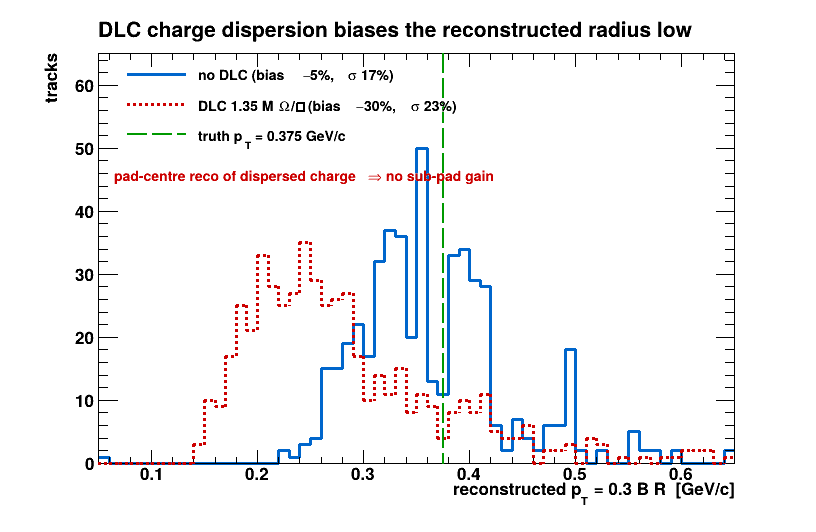
\includegraphics[width=\linewidth]{figs/dlc_effect.png}
\column{0.48\textwidth}
The resistive DLC anode is \textbf{always active}. Its charge dispersion ($\sigma\approx1.1$ mm) spreads each cluster over \textbf{$\sim$4$\times$ more pads} (36 $\to$ 145 pads/event).
\begin{itemize}
\item With \textbf{pad-centre} reconstruction (max-PSA), the dispersed charge broadens the arc and biases the fitted circle radius \alert{$\sim$30\% low} $\Rightarrow$ momentum bias $-20\%$, $\sigma$ worse.
\item A blunt amplitude threshold does \emph{not} fix it (overshoots, destabilises).
\end{itemize}
The sub-pad information DLC encodes is there --- but pad-centre hits throw it away.
\end{columns}
\end{frame}

\begin{frame}{Recovering the resolution --- three levers}
\begin{columns}
\column{0.54\textwidth}
\centering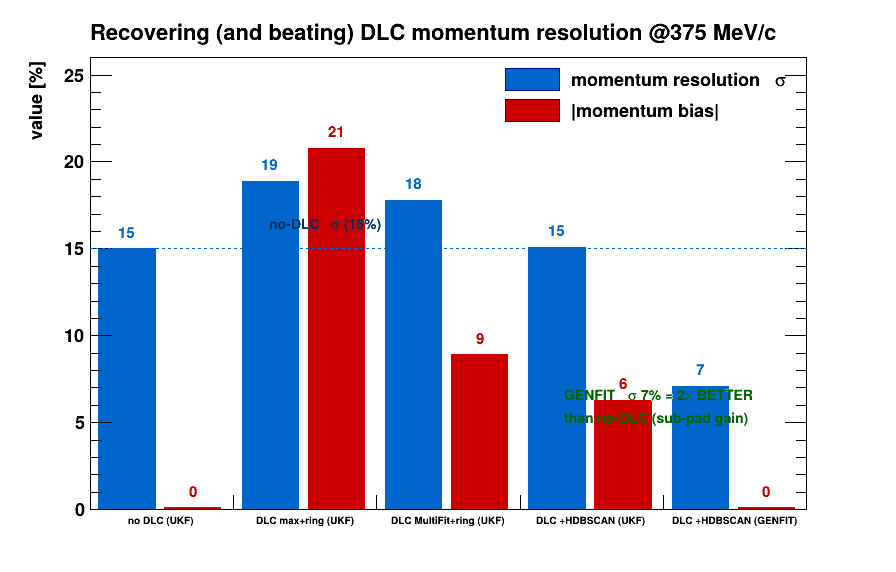
\includegraphics[width=\linewidth]{figs/dlc_ladder.png}
\column{0.46\textwidth}
Recover the sub-pad information by combining:
\begin{enumerate}
\item \textbf{AtPSAMultiFit} --- fitted pulse charge is a far better per-pad weight than the peak ADC \\ ($-21\% \to -9\%$ bias).
\item \textbf{HDBSCAN} --- cleanly clusters the dense dispersed band (TriplClust entangles it with its own failure modes).
\item \textbf{per-ring charge-weighted centroiding} --- one sub-pad point per annular ring.
\end{enumerate}
Together they return the momentum resolution to the no-DLC value.
\end{columns}
\end{frame}

\begin{frame}{What caused the bias --- and why the cure works}
\begin{columns}
\column{0.5\textwidth}
\textbf{Cause --- a reconstruction artefact, not physics:}
\begin{itemize}
\item DLC disperses the charge, but max-PSA reconstructs each fired pad as \textbf{one hit at its geometric centre}, discarding the sub-pad charge distribution.
\item A track's ionisation --- physically at a well-defined \emph{sub-pad} point --- becomes a $\sim$1--2 pad-wide \textbf{band} of pad-centre hits. The circle fit through the broadened band returns a systematically \alert{smaller radius} $\Rightarrow$ momentum biased low.
\item It is \emph{not} in the digitisation: the deposited-charge centroid is correct.
\end{itemize}
\column{0.5\textwidth}
\textbf{Cure --- recover the charge-weighted sub-pad centroid:}
\begin{itemize}
\item[1.] accurate \textbf{per-pad charge} (MultiFit fitted integral, not the biased peak ADC),
\item[2.] correct \textbf{clustering} of the dispersed pads (HDBSCAN),
\item[3.] the \textbf{charge-weighted centroid} itself (per-ring).
\end{itemize}
The bias shrinks \emph{monotonically} as the centroid gets more accurate ($-30\% \to -20\% \to -9\% \to -6\% \to 0$), vanishing when GENFIT weights the 0.3 mm centroids optimally.\\[.3em]
\textbf{Proof it is the sub-pad recovery:} same chain, DLC off $\sigma=19\%$ vs on $\sigma=7\%$ --- the charge spread is what \emph{enables} the sub-pad measurement.
\end{columns}
\end{frame}

\begin{frame}{UKF vs GENFIT with DLC --- the sub-pad win}
\centering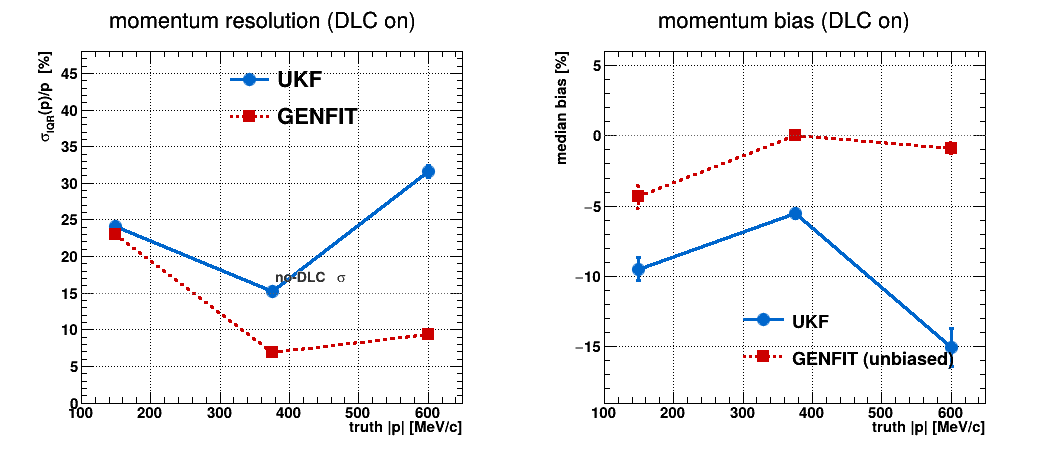
\includegraphics[height=.52\textheight]{figs/dlc_ukf_genfit.png}\\[.2em]
{\footnotesize Winning chain (MultiFit + HDBSCAN + per-ring), DLC on.\quad
\begin{tabular}{lcccc}\toprule
@375 MeV/c & momentum bias & momentum $\sigma$ & $\theta$ $\sigma$ & vertex $\sigma_z$\\\midrule
UKF & $-6.3\%$ & 15.1\% & 1.84$^\circ$ & 0.50 mm\\
GENFIT & \textbf{$-0.1\%$} & \textbf{7.1\%} & 1.76$^\circ$ & 0.47 mm\\\bottomrule
\end{tabular}}\\[.3em]
{\small \textbf{GENFIT} --- told the ring centroids are accurate to 0.3 mm --- exploits the sub-pad charge fully: \textbf{unbiased, $\sigma$ 7\%}, twice as good as without DLC, and 7--9\% across 375--600 MeV/c. Control (same chain, DLC off$\to$on): GENFIT $19\% \to 7\%$ --- the gain is genuinely DLC.}
\end{frame}

\begin{frame}{Momentum residual after full correction (DLC on)}
\begin{columns}
\column{0.58\textwidth}
\centering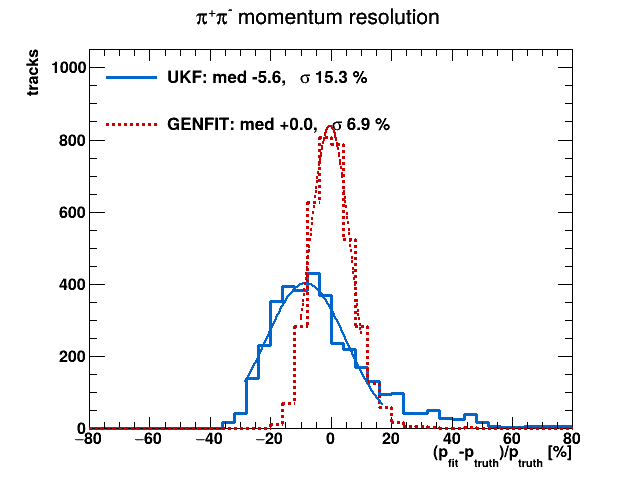
\includegraphics[width=\linewidth]{figs/res_pi_dlc_dp.png}
\column{0.42\textwidth}
The reconstructed momentum residual for the winning chain, DLC on, \emph{after} the Cu/Al material correction \emph{and} the DLC sub-pad recovery (500 events).
\begin{itemize}
\item \textbf{GENFIT} peaks cleanly at zero --- median $-0.1\%$, $\sigma$ \textbf{7.2\%}.
\item \textbf{UKF} is broader ($\sigma$ 15\%) and shifted ($-6\%$).
\end{itemize}
Both are unbiased/tight in $\theta$ ($1.84^\circ$) and vertex-$z$ ($\sigma_z\,0.47$--$0.50$ mm). This is the final, corrected performance.
\end{columns}
\end{frame}

\begin{frame}{Performance summary --- optimal chain, DLC on}
\centering
\textbf{Back-to-back $\pi^+\pi^-$ at 375 MeV/c} (MultiFit + HDBSCAN + per-ring + DLC)\\[.4em]
\begin{tabular}{lcc}\toprule
metric & UKF & GENFIT\\\midrule
tracking efficiency & 99.7\% & 99.7\%\\
fitting efficiency & 100\% & 100\%\\
momentum bias & $-5.6\%$ & \textbf{$+0.0\%$}\\
momentum resolution $\sigma$ & 15.3\% & \textbf{6.9\%}\\
polar-angle $\sigma$ & 2.0$^\circ$ & 2.0$^\circ$\\
vertex $\sigma_z$ & 0.50 mm & \textbf{0.48 mm}\\
charge-sign accuracy & 99.5\% & 99.6\%\\\bottomrule
\end{tabular}
\qquad
\begin{tabular}{lccc}\toprule
$|p|$ & tracking & fitting & GENFIT $\sigma$/bias\\\midrule
150 & 72\% & 99\% & 23\% / $-4.3\%$\\
375 & \textbf{99.7\%} & \textbf{100\%} & \textbf{6.9\% / $+0.0\%$}\\
600 & 100\% & 93\% & 9.4\% / $-0.9\%$\\\bottomrule
\end{tabular}\\[.5em]
{\small Tracking is limited at low $p$ (over-segmentation of tight curls); fitting at high $p$ (near-straight tracks). At the nominal 375 MeV/c everything is $\sim$100\%.}
\end{frame}

\begin{frame}{Particle ID: $\pi^+$/$\pi^-$ separation (DLC on)}
\begin{columns}
\column{0.56\textwidth}
\centering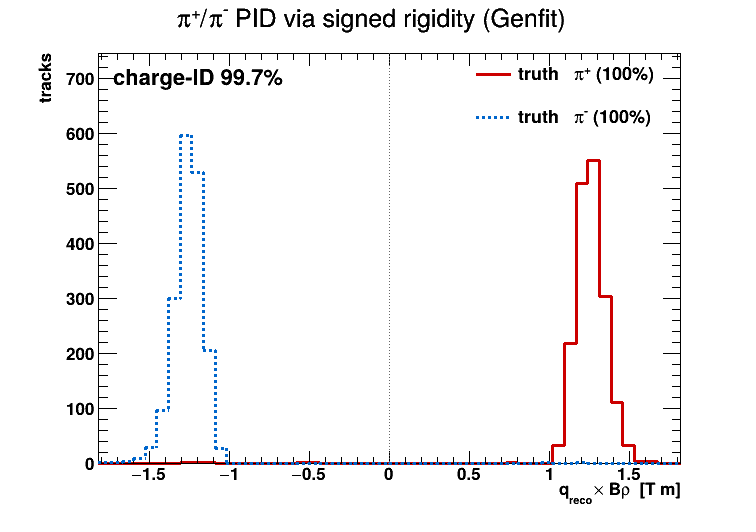
\includegraphics[width=\linewidth]{figs/pid_pipm_dlc.png}
\column{0.44\textwidth}
$\pi^+$ and $\pi^-$ have identical mass, so they separate purely by \textbf{charge sign} --- the signed rigidity $q\,B\rho$.\\[.5em]
With the DLC sub-pad momentum resolution (GENFIT) the peaks are \textbf{tight} ($\sigma=0.09$ T\,m at $\pm1.25$): charge-ID \textbf{99.7\%}, separation power \textbf{$S=14.5\,\sigma$} --- up from $5.9\,\sigma$ without DLC.\\[.5em]
Better momentum resolution $\Rightarrow$ better particle ID: another DLC dividend.
\end{columns}
\end{frame}

\begin{frame}{Pattern recognition --- examples (DLC on)}
\centering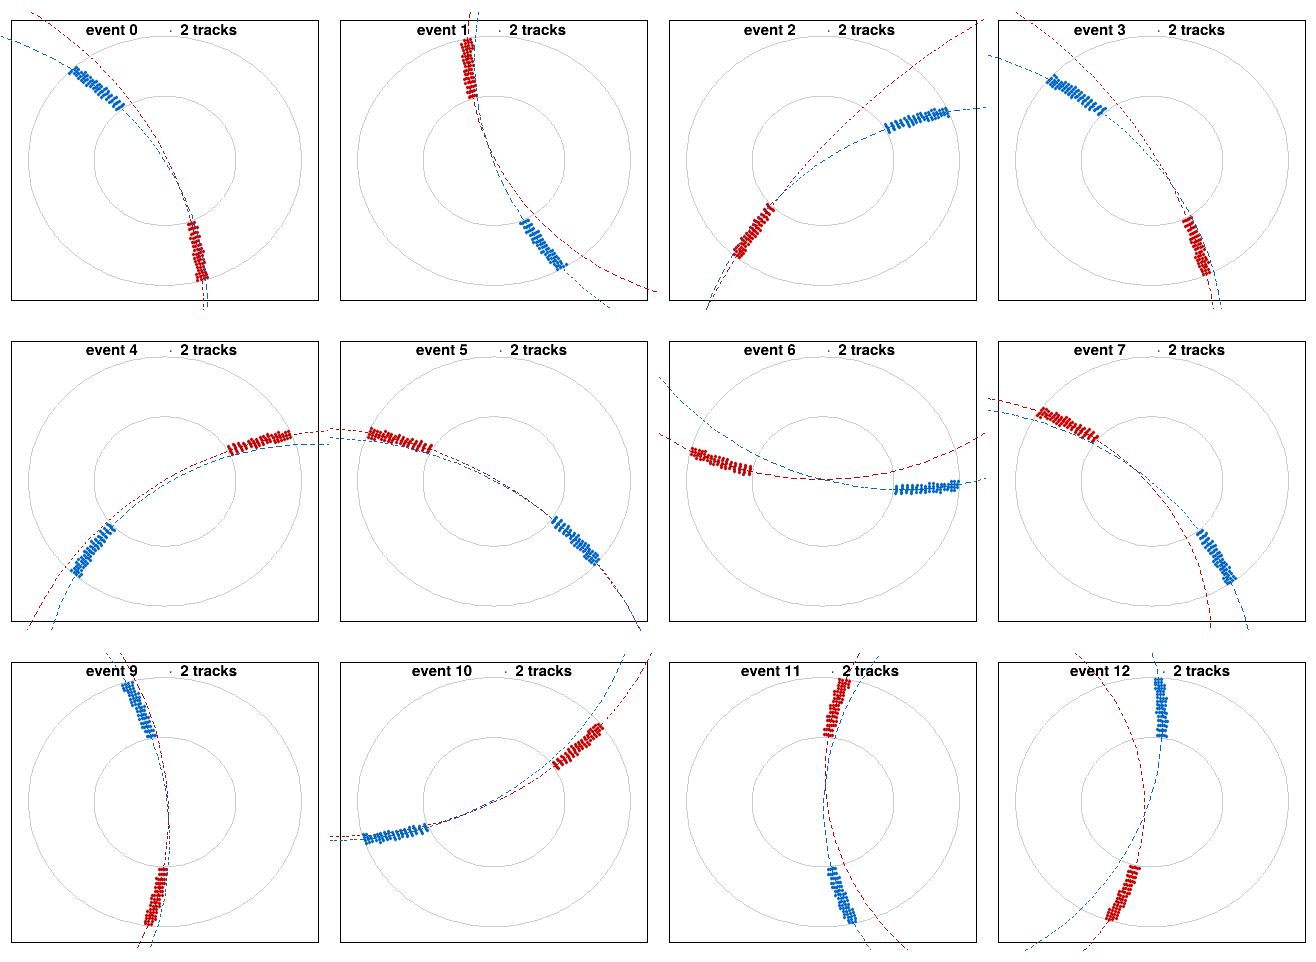
\includegraphics[height=.80\textheight]{figs/pra_examples.png}\\
{\small Twelve events: hits coloured per track candidate with the PRA circle fit (dashed) overlaid. DLC-dispersed charge gives the fattened hit bands.}
\end{frame}

\begin{frame}{Kalman fits --- examples (DLC on)}
\centering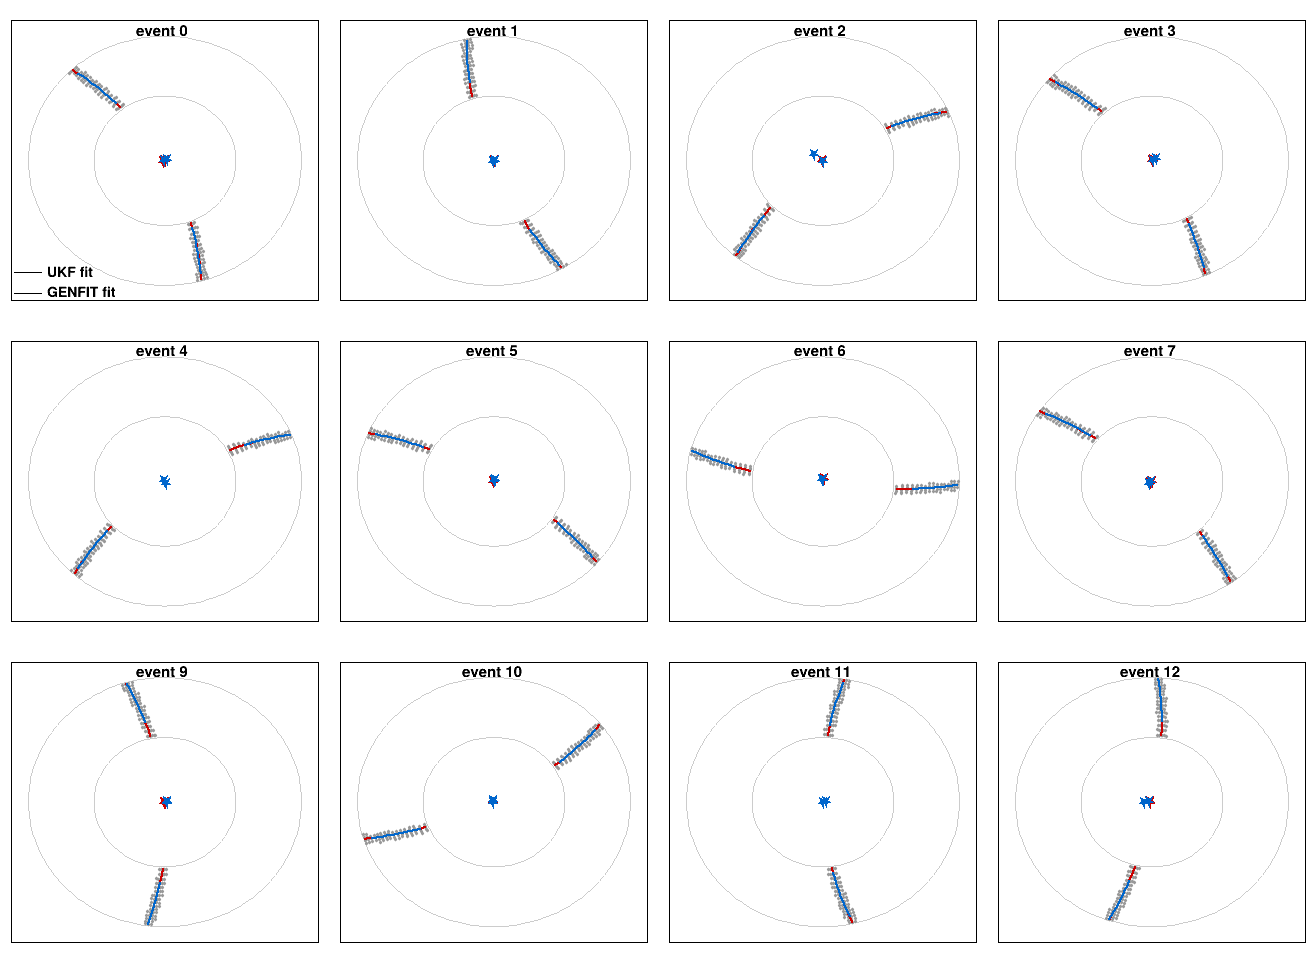
\includegraphics[height=.80\textheight]{figs/fit_examples.png}\\
{\small Twelve events: reconstructed hits (grey) with the \textcolor{blue}{UKF} and \textcolor{red}{GENFIT} fitted trajectories; stars = back-extrapolated vertices, converging on the beam axis.}
\end{frame}

\begin{frame}{Conclusion: DLC is an advantage}
\begin{itemize}
\item The always-on DLC anode is a \textbf{momentum-resolution advantage}, not a cost --- \emph{if} its sub-pad charge is properly reconstructed.
\item Pad-centre reconstruction wastes it (biases momentum $-20\%$). The fix is \textbf{MultiFit PSA + HDBSCAN + per-ring charge-weighted clustering}.
\item \textbf{GENFIT} is the fitter of choice with DLC: unbiased, $\sigma\,7\%$ momentum at 375 MeV/c --- \textbf{2$\times$ better than without DLC}. Its tight 0.3 mm measurement model is justified only by DLC's real sub-pad information.
\end{itemize}
\vspace{.4em}
\begin{block}{Recommended production chain (DLC on)}
\centering \texttt{AtPSAMultiFit} $\to$ \texttt{HDBSCAN} $\to$ per-ring charge-weighting $\to$ \textbf{GENFIT}
\end{block}
\end{frame}

\end{document}
